\documentclass[11pt,a4paper]{report}

\usepackage[utf8]{inputenc}
\usepackage[T1]{fontenc}
\usepackage[margin=1in]{geometry}
\usepackage{graphicx}
\usepackage{xcolor}
\usepackage{listings}
\usepackage{hyperref}
\usepackage{booktabs}
\usepackage{enumitem}
\usepackage{fancyhdr}
\usepackage{titlesec}
\usepackage{tocloft}
\usepackage{amsmath}
\usepackage{tikz}
\usepackage{multicol}
\usepackage{float}

% Colors (matching software_docs.tex)
\definecolor{codebackground}{RGB}{245,245,245}
\definecolor{codecomment}{RGB}{0,128,0}
\definecolor{codekeyword}{RGB}{0,0,180}
\definecolor{codestring}{RGB}{163,21,21}
\definecolor{linkcolor}{RGB}{0,80,160}
\definecolor{chaptercolor}{RGB}{40,60,100}
\definecolor{pincolor}{RGB}{200,60,60}
\definecolor{muxcolor}{RGB}{60,120,200}
\definecolor{sensorcolor}{RGB}{60,160,60}
\definecolor{warnbg}{RGB}{255,240,230}

% Hyperref setup
\hypersetup{
    colorlinks=true,
    linkcolor=linkcolor,
    urlcolor=linkcolor,
    citecolor=linkcolor,
    pdftitle={Kirin Hardware Integration Guide},
    pdfauthor={Strydr Silverberg},
}

% Code listing style
\lstdefinestyle{codestyle}{
    backgroundcolor=\color{codebackground},
    basicstyle=\ttfamily\small,
    breakatwhitespace=false,
    breaklines=true,
    captionpos=b,
    commentstyle=\color{codecomment}\itshape,
    keywordstyle=\color{codekeyword}\bfseries,
    stringstyle=\color{codestring},
    numberstyle=\tiny\color{gray},
    numbers=left,
    numbersep=8pt,
    showspaces=false,
    showstringspaces=false,
    showtabs=false,
    tabsize=4,
    frame=single,
    framerule=0.5pt,
    rulecolor=\color{gray!50},
}
\lstset{style=codestyle}

% Chapter and section styling
\titleformat{\chapter}[display]
    {\normalfont\huge\bfseries\color{chaptercolor}}
    {\chaptertitlename\ \thechapter}{20pt}{\Huge}
\titlespacing*{\chapter}{0pt}{0pt}{30pt}

% Header and footer
\pagestyle{fancy}
\fancyhf{}
\fancyhead[L]{\leftmark}
\fancyhead[R]{\thepage}
\renewcommand{\headrulewidth}{0.4pt}

% Note box
\newcommand{\notebox}[1]{%
    \begin{center}
    \fcolorbox{gray}{gray!10}{%
        \parbox{0.9\textwidth}{\textbf{Note:} #1}
    }
    \end{center}
}

% Warning box
\newcommand{\warningbox}[1]{%
    \begin{center}
    \fcolorbox{red!70}{red!10}{%
        \parbox{0.9\textwidth}{\textbf{Warning:} #1}
    }
    \end{center}
}

% Tip box
\newcommand{\tipbox}[1]{%
    \begin{center}
    \fcolorbox{green!60!black}{green!5}{%
        \parbox{0.9\textwidth}{\textbf{Tip:} #1}
    }
    \end{center}
}

%------------------------------------------------------------------------------
% Document Information
%------------------------------------------------------------------------------
\title{%
    \vspace{-1cm}
    \rule{\textwidth}{1pt}\\[0.5cm]
    {\Huge\bfseries Kirin}\\[0.3cm]
    {\Large Hardware Integration Guide}\\[0.3cm]
    \rule{\textwidth}{1pt}\\[1cm]
    {\large Connecting the Raspberry Pi to the Physical Chess Board}
}
\author{Strydr Silverberg \& Colin Dake\\\\Colorado School of Mines\\2026 ProtoFund}
\date{\today}

\begin{document}

\maketitle
\thispagestyle{empty}

\vfill
\begin{center}
    \textit{A step-by-step guide to wiring, configuring, and testing the Kirin\\
    autonomous chess system on a Raspberry Pi.}
\end{center}
\vfill

\newpage
\tableofcontents
\newpage

%==============================================================================
\chapter{Overview}
%==============================================================================

\section{What This Document Covers}

This guide walks through the complete process of connecting the Kirin software to the physical chess board hardware. By the end, you will have a Raspberry Pi running the Kirin engine, reading 96 hall effect sensors through multiplexers, and controlling a gantry system via GRBL over serial.

The system has three hardware subsystems that connect to the Pi:

\begin{enumerate}
    \item \textbf{Hall Effect Sensors (96 total)} --- detect piece presence on the board and in the two storage zones. Read through 6 multiplexers using 10 GPIO pins.
    \item \textbf{GRBL Gantry Controller} --- moves pieces on the physical board via an electromagnet on a 2-axis gantry. Communicates over USB serial.
    \item \textbf{Electromagnet} --- controlled by the GRBL board via the spindle output (M3/M5 commands).
\end{enumerate}

\section{System Architecture}

\begin{center}
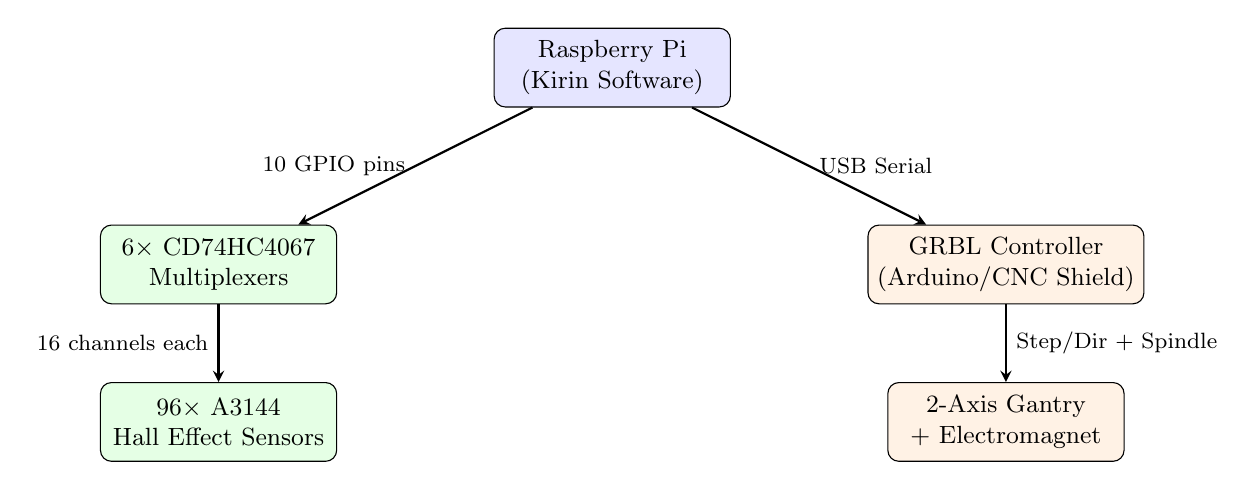
\begin{tikzpicture}[
    box/.style={draw, rounded corners, minimum width=3cm, minimum height=1cm, align=center, font=\small},
    arr/.style={->, thick, >=stealth}
]
    % Pi
    \node[box, fill=blue!10] (pi) at (0, 0) {Raspberry Pi\\(Kirin Software)};
    
    % Sensors
    \node[box, fill=green!10] (mux) at (-5, -2.5) {6$\times$ CD74HC4067\\Multiplexers};
    \node[box, fill=green!10] (sensors) at (-5, -4.5) {96$\times$ A3144\\Hall Effect Sensors};
    
    % GRBL
    \node[box, fill=orange!10] (grbl) at (5, -2.5) {GRBL Controller\\(Arduino/CNC Shield)};
    \node[box, fill=orange!10] (gantry) at (5, -4.5) {2-Axis Gantry\\+ Electromagnet};
    
    % Connections
    \draw[arr] (pi) -- node[left, font=\footnotesize] {10 GPIO pins} (mux);
    \draw[arr] (mux) -- node[left, font=\footnotesize] {16 channels each} (sensors);
    \draw[arr] (pi) -- node[right, font=\footnotesize] {USB Serial} (grbl);
    \draw[arr] (grbl) -- node[right, font=\footnotesize] {Step/Dir + Spindle} (gantry);
\end{tikzpicture}
\end{center}

\section{Prerequisites}

\begin{table}[H]
\centering
\begin{tabular}{ll}
\toprule
\textbf{Item} & \textbf{Details} \\
\midrule
Raspberry Pi & Pi 4 or Pi 5 (any RAM) \\
OS & Raspberry Pi OS (64-bit recommended) \\
Compiler & GCC with C++17 support \\
CMake & Version 3.10 or later \\
libgpiod & \texttt{sudo apt install libgpiod-dev} \\
Serial port & USB connection to GRBL controller \\
\bottomrule
\end{tabular}
\caption{Required components}
\end{table}


%==============================================================================
\chapter{Building the Software}
%==============================================================================

\section{Clone and Build}

\begin{lstlisting}[language=bash]
# Clone the repository
git clone https://github.com/your-repo/kirin.git
cd kirin

# Create build directory
mkdir build && cd build

# Configure with GPIO support
cmake .. -DCMAKE_BUILD_TYPE=Release \
         -DCMAKE_CXX_FLAGS="-DHAS_GPIOD"

# Build
make -j$(nproc)
\end{lstlisting}

\warningbox{The \texttt{-DHAS\_GPIOD} flag is essential. Without it, the board scanner compiles in stub mode and all GPIO calls are no-ops. The build will succeed either way, but the sensors will not work without this flag.}

\section{Install Dependencies}

\begin{lstlisting}[language=bash]
# Install libgpiod for GPIO access (no root required at runtime)
sudo apt install libgpiod-dev

# Verify installation
dpkg -l | grep libgpiod
\end{lstlisting}

\section{Run the Tests}

Before connecting any hardware, verify the software is correct:

\begin{lstlisting}[language=bash]
cd build

# Run all tests
ctest --output-on-failure

# Or run individually
./board_scanner_test     # Sensor move detection logic (62 tests)
./game_controller_test   # Engine-to-physical bridge
./board_interpreter_test # Path planning
./engine_test            # Engine validation
./captured_piece_test    # Capture encoding
\end{lstlisting}

All tests should pass. The board scanner tests run entirely in simulation mode and do not require GPIO hardware.


%==============================================================================
\chapter{Wiring the Hall Effect Sensors}
%==============================================================================

\section{Sensor Overview}

The system uses 96 A3144 hall effect sensors to detect the presence of magnets embedded in the chess pieces. The sensors are digital (output LOW when a magnet is detected, HIGH when no magnet is present) and require a 10K pull-up resistor each.

The 96 sensors are organized as follows:

\begin{table}[H]
\centering
\begin{tabular}{clcl}
\toprule
\textbf{Mux} & \textbf{Coverage} & \textbf{Channels} & \textbf{GPIO (SIG)} \\
\midrule
0 & Board ranks 8--7 (a8--h7) & 0--15 & GPIO 5 \\
1 & Board ranks 6--5 (a6--h5) & 0--15 & GPIO 6 \\
2 & Board ranks 4--3 (a4--h3) & 0--15 & GPIO 13 \\
3 & Board ranks 2--1 (a2--h1) & 0--15 & GPIO 19 \\
4 & Black storage zone (16 slots) & 0--15 & GPIO 26 \\
5 & White storage zone (16 slots) & 0--15 & GPIO 16 \\
\bottomrule
\end{tabular}
\caption{Multiplexer assignments}
\end{table}

\section{Multiplexer Wiring}

All six CD74HC4067 multiplexers share four address/select lines. The Pi sets these four lines (S0--S3) to select a channel (0--15), then reads the SIG output from each mux simultaneously.

\subsection{Shared Select Lines (Pi $\rightarrow$ All 6 Muxes)}

\begin{table}[H]
\centering
\begin{tabular}{ccc}
\toprule
\textbf{Select Line} & \textbf{Pi GPIO (BCM)} & \textbf{Mux Pin} \\
\midrule
S0 & GPIO 17 & Pin 10 (S0) on all muxes \\
S1 & GPIO 27 & Pin 11 (S1) on all muxes \\
S2 & GPIO 22 & Pin 14 (S2) on all muxes \\
S3 & GPIO 23 & Pin 15 (S3) on all muxes \\
\bottomrule
\end{tabular}
\caption{Select line wiring (active on all 6 muxes)}
\end{table}

\subsection{Signal Output Lines (Each Mux $\rightarrow$ Pi)}

Each mux has a single SIG output that goes to its own GPIO pin on the Pi:

\begin{table}[H]
\centering
\begin{tabular}{ccl}
\toprule
\textbf{Mux} & \textbf{SIG $\rightarrow$ Pi GPIO} & \textbf{Direction} \\
\midrule
0 & GPIO 5 & Input (Pi reads) \\
1 & GPIO 6 & Input \\
2 & GPIO 13 & Input \\
3 & GPIO 19 & Input \\
4 & GPIO 26 & Input \\
5 & GPIO 16 & Input \\
\bottomrule
\end{tabular}
\caption{Signal output wiring}
\end{table}

\subsection{Power and Enable}

\begin{itemize}
    \item Connect VCC on each mux to 3.3V (the Pi's GPIO operates at 3.3V).
    \item Connect GND on each mux to the Pi's GND.
    \item Connect the EN (enable) pin on each mux to GND (active-low enable, so grounding it keeps the mux always enabled).
\end{itemize}

\warningbox{Do not power the muxes from 5V. The CD74HC4067 will work at 3.3V, and connecting a 5V signal to the Pi's GPIO pins can damage the Pi.}

\section{Sensor-to-Channel Mapping}

Within each board mux, the 16 channels map to squares as follows:

\begin{table}[H]
\centering
\begin{tabular}{cl|cl}
\toprule
\textbf{Channel} & \textbf{Square (Mux 0)} & \textbf{Channel} & \textbf{Square (Mux 0)} \\
\midrule
0 & a8 & 8 & a7 \\
1 & b8 & 9 & b7 \\
2 & c8 & 10 & c7 \\
3 & d8 & 11 & d7 \\
4 & e8 & 12 & e7 \\
5 & f8 & 13 & f7 \\
6 & g8 & 14 & g7 \\
7 & h8 & 15 & h7 \\
\bottomrule
\end{tabular}
\caption{Channel-to-square mapping (Mux 0 shown; pattern repeats for Mux 1--3)}
\end{table}

The pattern is: channels 0--7 map to the higher rank (file a through h), channels 8--15 map to the lower rank. For storage muxes (4 and 5), channels 0--7 are back-rank piece slots and channels 8--15 are pawn slots.

\tipbox{If your physical wiring doesn't match this channel order, you have two options: re-wire the sensors, or modify \texttt{toSquareIndex()} in \texttt{board\_scanner.cpp} to match your actual wiring. Re-wiring is usually easier.}

\section{A3144 Sensor Circuit}

Each A3144 sensor has three pins: VCC, GND, and OUTPUT. The output is open-collector, so it needs a pull-up resistor:

\begin{center}
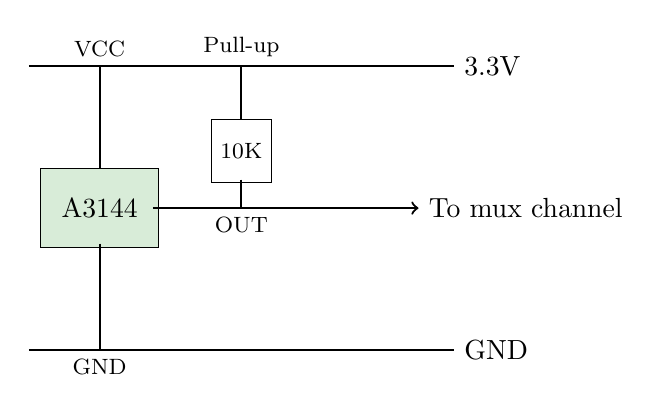
\begin{tikzpicture}[scale=0.9]
    % VCC rail
    \draw[thick] (0, 4) -- (6, 4) node[right] {3.3V};
    
    % Sensor
    \draw[thick] (1, 4) -- (1, 2.5);
    \node[draw, minimum width=1.5cm, minimum height=1cm, fill=sensorcolor!20] at (1, 2) {A3144};
    \draw[thick] (1, 1.5) -- (1, 0);
    \draw[thick] (1.75, 2) -- (3, 2);
    
    % Pull-up resistor
    \draw[thick] (3, 4) -- (3, 3.2);
    \node[draw, minimum width=0.4cm, minimum height=0.8cm, fill=white] at (3, 2.8) {\footnotesize 10K};
    \draw[thick] (3, 2.4) -- (3, 2);
    
    % To mux
    \draw[thick, ->] (3, 2) -- (5.5, 2) node[right] {To mux channel};
    
    % GND rail
    \draw[thick] (0, 0) -- (6, 0) node[right] {GND};
    
    % Labels
    \node[above] at (1, 4) {\footnotesize VCC};
    \node[below] at (1, 0) {\footnotesize GND};
    \node[above] at (3, 4) {\footnotesize Pull-up};
    \node[below] at (3, 2) {\footnotesize OUT};
\end{tikzpicture}
\end{center}

When a magnet is present, the A3144 pulls its output LOW. When no magnet is present, the pull-up resistor holds the output HIGH. The software inverts this logic: LOW = piece present, HIGH = empty.


%==============================================================================
\chapter{Connecting the Gantry}
%==============================================================================

\section{GRBL Connection}

The gantry controller (typically an Arduino Uno with a CNC shield running GRBL firmware) connects to the Pi via USB. This appears as a serial port, usually \texttt{/dev/ttyUSB0} or \texttt{/dev/ttyACM0}.

\begin{lstlisting}[language=bash]
# Find the serial port
ls /dev/ttyUSB* /dev/ttyACM*

# Check permissions (your user must be in the 'dialout' group)
groups $USER | grep dialout

# If not in the group:
sudo usermod -aG dialout $USER
# Log out and back in for this to take effect
\end{lstlisting}

\section{GRBL Settings}

The Kirin software communicates at 115200 baud (GRBL default). Verify the GRBL settings match the physical gantry dimensions. Connect to GRBL with a serial terminal to check:

\begin{lstlisting}[language=bash]
# Connect with minicom (or screen, picocom, etc.)
minicom -D /dev/ttyUSB0 -b 115200

# In the GRBL console, type:
$$
# This prints all settings
\end{lstlisting}

Key settings to verify:

\begin{table}[H]
\centering
\begin{tabular}{clp{7cm}}
\toprule
\textbf{Setting} & \textbf{Parameter} & \textbf{Notes} \\
\midrule
\$100 & X steps/inch & Must match your stepper + lead screw \\
\$101 & Y steps/inch & Must match your stepper + lead screw \\
\$110 & X max rate (in/min) & Software uses 1000 in/min default \\
\$111 & Y max rate (in/min) & Must be $\geq$ 1000 \\
\$120 & X acceleration (in/s$^2$) & Start with 10, increase after testing \\
\$121 & Y acceleration (in/s$^2$) & Start with 10, increase after testing \\
\$130 & X max travel (in) & Should be $\geq$ 22 (rail travel) \\
\$131 & Y max travel (in) & Should be $\geq$ 22 \\
\$22 & Homing cycle & Set to 1 (enabled) \\
\bottomrule
\end{tabular}
\caption{Critical GRBL settings}
\end{table}

\section{Electromagnet Control}

The electromagnet is controlled through GRBL's spindle output:

\begin{itemize}
    \item \texttt{M3} = Magnet ON (spindle CW --- repurposed for electromagnet)
    \item \texttt{M5} = Magnet OFF (spindle stop)
\end{itemize}

The CNC shield's spindle enable pin drives a MOSFET or relay that controls the electromagnet. Verify this works before running any game:

\begin{lstlisting}[language=bash]
# In the GRBL console:
M3     # Magnet should engage
G4 P2000  # Wait 2 seconds
M5     # Magnet should release
\end{lstlisting}

\section{Physical Coordinate System}

The software maps board squares to physical coordinates in inches. The board layout is:

\begin{center}
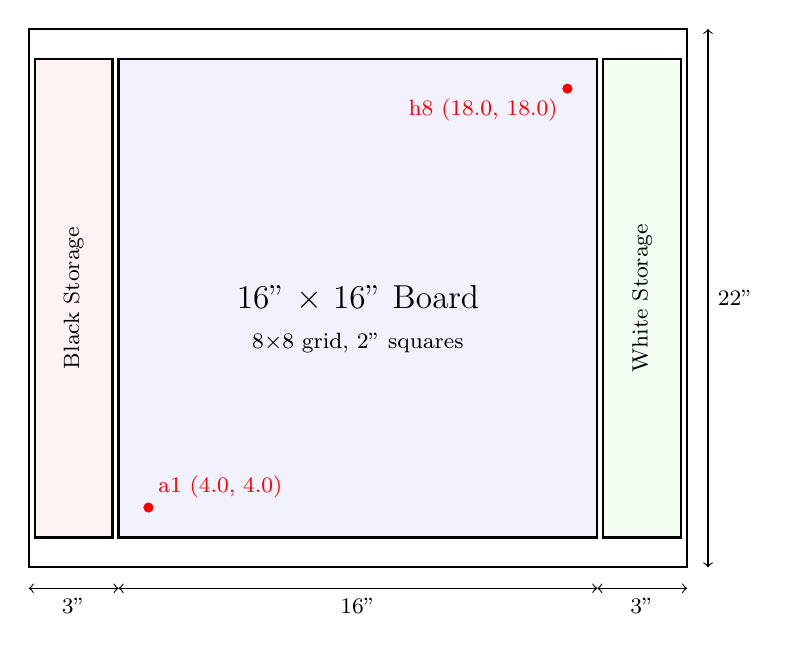
\begin{tikzpicture}[scale=0.38]
    % Rail
    \draw[thick] (0, 0) rectangle (22, 18);
    
    % Board
    \draw[thick, fill=blue!5] (3, 1) rectangle (19, 17);
    \node at (11, 9) {\large 16'' $\times$ 16'' Board};
    \node at (11, 7.5) {\footnotesize 8$\times$8 grid, 2'' squares};
    
    % Black storage
    \draw[thick, fill=red!5] (0.2, 1) rectangle (2.8, 17);
    \node[rotate=90] at (1.5, 9) {\footnotesize Black Storage};
    
    % White storage
    \draw[thick, fill=green!5] (19.2, 1) rectangle (21.8, 17);
    \node[rotate=90] at (20.5, 9) {\footnotesize White Storage};
    
    % Dimensions
    \draw[<->] (0, -0.7) -- (3, -0.7) node[midway, below] {\footnotesize 3''};
    \draw[<->] (3, -0.7) -- (19, -0.7) node[midway, below] {\footnotesize 16''};
    \draw[<->] (19, -0.7) -- (22, -0.7) node[midway, below] {\footnotesize 3''};
    \draw[<->] (22.7, 0) -- (22.7, 18) node[midway, right] {\footnotesize 22''};
    
    % a1 marker
    \filldraw[red] (4, 2) circle (0.15);
    \node[red, above right] at (4, 2) {\footnotesize a1 (4.0, 4.0)};
    
    % h8 marker
    \filldraw[red] (18, 16) circle (0.15);
    \node[red, below left] at (18, 16) {\footnotesize h8 (18.0, 18.0)};
\end{tikzpicture}
\end{center}

The coordinate system origin (0,0) is at the bottom-left of the rail travel. Square a1 is centered at (4.0'', 4.0'') and each square is 2'' wide. Verify that the gantry homes to (0,0) and that commanding \texttt{G1 X4.0 Y4.0} positions the magnet over the center of a1.


%==============================================================================
\chapter{First Power-On Procedure}
%==============================================================================

\section{Step 1: Verify GPIO Chip}

The Pi 5 and Pi 4 use different GPIO chip paths. The software auto-detects, but verify:

\begin{lstlisting}[language=bash]
# Pi 5:
ls /dev/gpiochip4  # Should exist

# Pi 4 and earlier:
ls /dev/gpiochip0  # Should exist

# List all GPIO chips:
gpiodetect
\end{lstlisting}

\section{Step 2: Start Kirin in Physical Mode}

\begin{lstlisting}[language=bash]
cd build
./kirin --physical /dev/ttyUSB0
\end{lstlisting}

You should see:

\begin{lstlisting}[language=bash, numbers=none]
Kirin Autonomous Chess System v0.3
Physical Board Mode

Connecting to gantry on /dev/ttyUSB0...
Connected to gantry on /dev/ttyUSB0
Initializing board scanner...
[SCANNER] GPIO initialized successfully (6 muxes: 4 board + 2 storage)
  Select lines: GPIO 17, 27, 22, 23
  Board muxes:  GPIO 5, 6, 13, 19
  Storage muxes: GPIO 26 (black), 16 (white)
Board scanner initialized
Homing gantry...
Homing complete

Ready. Type 'help' for commands.
\end{lstlisting}

If the scanner fails to initialize, check your wiring and ensure \texttt{-DHAS\_GPIOD} was used during compilation.

\section{Step 3: Run Sensor Diagnostics}

\begin{lstlisting}[language=bash, numbers=none]
kirin> diag
\end{lstlisting}

This reads every sensor individually and prints the result. Walk through each square with a magnet (or chess piece) and verify:

\begin{itemize}
    \item Each channel maps to the correct square
    \item ``PIECE'' appears when the magnet is present, ``empty'' when removed
    \item No stuck sensors (always reading PIECE or always empty)
    \item Storage zone sensors respond correctly
\end{itemize}

\section{Step 4: Quick Scan}

Place all 32 pieces on the board in the starting position, then:

\begin{lstlisting}[language=bash, numbers=none]
kirin> scan
\end{lstlisting}

You should see:

\begin{lstlisting}[language=bash, numbers=none]
  Sensor Scan:
    a b c d e f g h
  8 # # # # # # # # 8
  7 # # # # # # # # 7
  6 . . . . . . . . 6
  5 . . . . . . . . 5
  4 . . . . . . . . 4
  3 . . . . . . . . 3
  2 # # # # # # # # 2
  1 # # # # # # # # 1
    a b c d e f g h
  Pieces detected: 32
\end{lstlisting}

If any squares are wrong, re-check the wiring for that mux/channel.

\section{Step 5: Test the Gantry}

\begin{lstlisting}[language=bash, numbers=none]
kirin> test
\end{lstlisting}

This moves the gantry to e4, then d5, engages and disengages the magnet, and returns home. Watch for:

\begin{itemize}
    \item Smooth motion with no skipped steps
    \item Correct positioning over the square centers
    \item Magnet picks up and releases cleanly
    \item No collisions with pieces or board edges
\end{itemize}

\section{Step 6: Gantry Coordinate Calibration}

If the gantry doesn't align with the square centers, you need to adjust either the GRBL steps/inch settings or the software constants. Place a piece on a1 and command:

\begin{lstlisting}[language=bash, numbers=none]
kirin> home
\end{lstlisting}

Then type \texttt{test}. The gantry should move to e4 (center of the board). If it's offset, adjust \texttt{A1\_CENTER\_X} and \texttt{A1\_CENTER\_Y} in \texttt{gantry\_controller.h}, or recalibrate your GRBL \$100/\$101 steps/inch settings.

\tipbox{Get a1 and h8 aligned first. Since the coordinate system is linear, if these two corners are correct, all 64 squares will be correct.}


%==============================================================================
\chapter{Running Your First Game}
%==============================================================================

\section{Stage 1: Manual Move Entry (No Sensors)}

Start with manual move input to verify the gantry executes moves correctly:

\begin{lstlisting}[language=bash, numbers=none]
kirin> newgame black
\end{lstlisting}

This sets up the board (gantry moves all pieces from storage to starting squares), then the engine plays black. You type your moves:

\begin{lstlisting}[language=bash, numbers=none]
kirin> move e2e4
kirin> move d2d4
kirin> move g1f3
\end{lstlisting}

After each of your moves, the engine will think and physically move a piece in response. Watch for correct piece movement, especially during captures (the captured piece should go to the correct storage slot).

\section{Stage 2: Sensor-Based Play}

Once manual mode works, switch to the full sensor experience:

\begin{lstlisting}[language=bash, numbers=none]
kirin> play black
\end{lstlisting}

Now make your moves by physically moving pieces on the board. The system will detect your move automatically. The terminal will show:

\begin{lstlisting}[language=bash, numbers=none]
Move 1. -- Your turn. Make your move on the board.
Waiting for your move...
Detected move: e2e4
\end{lstlisting}

\subsection{What to Test}

\begin{enumerate}
    \item \textbf{Normal moves}: Pick up a pawn, place it on a new square.
    \item \textbf{Pondering}: Pick up a piece, hold it for 10+ seconds, put it back. The system should \emph{not} commit a move.
    \item \textbf{Take-back}: Pick up one piece, put it back, pick up a different piece and move it. Only the final move should register.
    \item \textbf{Captures}: Pick up the opponent's piece, place it in the storage zone, then move your piece to the vacated square.
    \item \textbf{Castling}: Move the king two squares, then move the rook. The system waits until both pieces are in their final positions.
    \item \textbf{Illegal state}: Move a piece to an illegal square. After 10 seconds, the system will alert you.
\end{enumerate}

\section{Stage 3: Full Game}

Play a complete game to checkmate or stalemate. The system will announce the result:

\begin{lstlisting}[language=bash, numbers=none]
==============================
  CHECKMATE -- White wins!
==============================
\end{lstlisting}


%==============================================================================
\chapter{Troubleshooting}
%==============================================================================

\section{Sensor Issues}

\begin{table}[H]
\centering
\begin{tabular}{p{5cm}p{9cm}}
\toprule
\textbf{Symptom} & \textbf{Solution} \\
\midrule
All sensors read empty & Check mux power (3.3V), verify EN pin is grounded, check select line wiring \\
\addlinespace
One mux reads all empty & Check that mux's SIG output wire to the Pi GPIO pin \\
\addlinespace
Random noise / flickering & Increase \texttt{DEBOUNCE\_SCANS} (default 3) or \texttt{DEBOUNCE\_DELAY\_MS} (default 50ms) in \texttt{board\_scanner.h} \\
\addlinespace
Sensors read wrong squares & Your channel-to-square wiring doesn't match the expected layout. Run \texttt{diag} and compare against the mapping table. Either re-wire or modify \texttt{toSquareIndex()} \\
\addlinespace
Sensors trigger from gantry magnet & The gantry electromagnet is interfering with nearby hall sensors. Add shielding around the gantry magnet, increase debounce, or only scan when the gantry is idle \\
\addlinespace
Scanner init fails & Verify \texttt{libgpiod-dev} is installed and the build used \texttt{-DHAS\_GPIOD}. Check that the GPIO chip exists (\texttt{/dev/gpiochip4} on Pi 5, \texttt{/dev/gpiochip0} on Pi 4) \\
\bottomrule
\end{tabular}
\caption{Common sensor issues}
\end{table}

\section{Gantry Issues}

\begin{table}[H]
\centering
\begin{tabular}{p{5cm}p{9cm}}
\toprule
\textbf{Symptom} & \textbf{Solution} \\
\midrule
``Failed to connect to gantry'' & Check USB cable, verify serial port path (\texttt{ls /dev/ttyUSB*}), ensure user is in \texttt{dialout} group \\
\addlinespace
Homing fails & Verify limit switches are connected and GRBL setting \$22=1 (homing enabled) \\
\addlinespace
Gantry moves to wrong position & Recalibrate GRBL steps/inch (\$100, \$101) or adjust \texttt{A1\_CENTER\_X}/\texttt{A1\_CENTER\_Y} in the software \\
\addlinespace
Magnet doesn't engage & Check GRBL spindle output wiring, test with \texttt{M3}/\texttt{M5} in a serial console \\
\addlinespace
Pieces dragged/knocked over & Reduce \texttt{FEED\_RATE} (default 1000 in/min), verify magnet strength is appropriate \\
\addlinespace
GRBL alarm triggered & The software auto-resets on alarm. Check error description in terminal output. Common cause: soft limits exceeded (piece near board edge) \\
\bottomrule
\end{tabular}
\caption{Common gantry issues}
\end{table}

\section{Move Detection Issues}

\begin{table}[H]
\centering
\begin{tabular}{p{5cm}p{9cm}}
\toprule
\textbf{Symptom} & \textbf{Solution} \\
\midrule
System doesn't detect my move & Verify the sensor under the destination square works (\texttt{diag}). Check that you placed the captured piece in storage (required for capture detection). \\
\addlinespace
System hangs waiting for move & If it's a rare ambiguous capture (queen can capture two different pieces from the same square), fall back to typed input: press Ctrl+C and use \texttt{move} command. \\
\addlinespace
``Board state not recognized'' alert & You've left the board in a state that doesn't correspond to any legal move for 10+ seconds. Fix piece placement. \\
\addlinespace
Board mismatch after engine move & The gantry dropped a piece. The system will show which squares are wrong. Fix the pieces manually and type \texttt{continue}. \\
\bottomrule
\end{tabular}
\caption{Common move detection issues}
\end{table}


%==============================================================================
\chapter{GPIO Pin Reference}
%==============================================================================

Complete pin assignment table using BCM (Broadcom) numbering:

\begin{table}[H]
\centering
\begin{tabular}{ccll}
\toprule
\textbf{BCM Pin} & \textbf{Direction} & \textbf{Function} & \textbf{Connects To} \\
\midrule
17 & Output & Select S0 & S0 on all 6 muxes \\
27 & Output & Select S1 & S1 on all 6 muxes \\
22 & Output & Select S2 & S2 on all 6 muxes \\
23 & Output & Select S3 & S3 on all 6 muxes \\
\addlinespace
5  & Input  & Mux 0 SIG & Board ranks 8--7 \\
6  & Input  & Mux 1 SIG & Board ranks 6--5 \\
13 & Input  & Mux 2 SIG & Board ranks 4--3 \\
19 & Input  & Mux 3 SIG & Board ranks 2--1 \\
26 & Input  & Mux 4 SIG & Black storage zone \\
16 & Input  & Mux 5 SIG & White storage zone \\
\bottomrule
\end{tabular}
\caption{All GPIO pin assignments (10 pins total)}
\end{table}

\notebox{These pin assignments can be overridden by passing custom arrays to the \texttt{BoardScanner} constructor. The defaults are defined in \texttt{board\_scanner.h}. If you need to change them, modify the \texttt{DEFAULT\_PIN\_*} constants and rebuild, or pass them at construction time.}

\begin{table}[H]
\centering
\begin{tabular}{cl}
\toprule
\textbf{Raspberry Pi Header Pin} & \textbf{BCM GPIO} \\
\midrule
Pin 11 & GPIO 17 (S0) \\
Pin 13 & GPIO 27 (S1) \\
Pin 15 & GPIO 22 (S2) \\
Pin 16 & GPIO 23 (S3) \\
Pin 29 & GPIO 5 (Mux 0) \\
Pin 31 & GPIO 6 (Mux 1) \\
Pin 33 & GPIO 13 (Mux 2) \\
Pin 35 & GPIO 19 (Mux 3) \\
Pin 37 & GPIO 26 (Mux 4) \\
Pin 36 & GPIO 16 (Mux 5) \\
\bottomrule
\end{tabular}
\caption{BCM to physical header pin mapping}
\end{table}


%==============================================================================
\chapter{Software Command Reference}
%==============================================================================

Quick reference for all commands available in physical mode:

\begin{table}[H]
\centering
\begin{tabular}{p{4.5cm}p{9.5cm}}
\toprule
\textbf{Command} & \textbf{Description} \\
\midrule
\texttt{play [white|black]} & Start a sensor-based game. Engine plays the specified color (default: white). Moves are detected automatically via hall effect sensors. \\
\addlinespace
\texttt{newgame [white|black]} & Start a game with manual (typed) move entry. Useful as a fallback if sensors aren't working. \\
\addlinespace
\texttt{move <uci>} & Manually enter a move in UCI format (e.g., \texttt{move e2e4}, \texttt{move e7e8q} for promotion). \\
\addlinespace
\texttt{go} & Engine makes one move. \\
\addlinespace
\texttt{scan} & Scan and display all 96 sensors (board + storage zones). \\
\addlinespace
\texttt{diag} & Run full sensor diagnostic --- reads each sensor individually with channel-by-channel output. \\
\addlinespace
\texttt{board} & Display the engine's internal board position. \\
\addlinespace
\texttt{physical} & Display the physical board occupancy tracking. \\
\addlinespace
\texttt{fen <fen>} & Set position from a FEN string. \\
\addlinespace
\texttt{home} & Home the gantry to (0,0). \\
\addlinespace
\texttt{test} & Run gantry hardware test (move to e4, d5, test magnet). \\
\addlinespace
\texttt{quit} & Exit the program. \\
\bottomrule
\end{tabular}
\caption{Physical mode commands}
\end{table}

%==============================================================================
\chapter{Tunable Parameters}
%==============================================================================

These constants in \texttt{board\_scanner.h} and \texttt{gantry\_controller.h} may need adjustment based on your specific hardware:

\begin{table}[H]
\centering
\begin{tabular}{p{4.5cm}cp{7cm}}
\toprule
\textbf{Constant} & \textbf{Default} & \textbf{Purpose} \\
\midrule
\texttt{MUX\_SETTLE\_US} & 10 $\mu$s & Time to wait after changing mux address before reading. Increase if readings are noisy. \\
\addlinespace
\texttt{DEBOUNCE\_SCANS} & 3 & Number of consecutive identical scans required before accepting a reading as stable. \\
\addlinespace
\texttt{DEBOUNCE\_DELAY\_MS} & 50 ms & Delay between debounce scans. Total debounce time = \texttt{SCANS} $\times$ \texttt{DELAY}. \\
\addlinespace
\texttt{POLL\_INTERVAL\_MS} & 20 ms & How often to poll sensors during \texttt{waitForLegalMove}. \\
\addlinespace
\texttt{ILLEGAL\_STATE\_ALERT\_MS} & 10,000 ms & How long the board can sit in an unrecognized state before alerting the player. \\
\addlinespace
\texttt{FEED\_RATE} & 1000 in/min & Gantry movement speed. Reduce if the gantry skips steps or knocks pieces over. \\
\addlinespace
\texttt{SQUARE\_SIZE} & 2.0 in & Physical size of each board square. \\
\addlinespace
\texttt{BOARD\_MARGIN} & 3.0 in & Distance from rail edge to first board square. \\
\bottomrule
\end{tabular}
\caption{Tunable hardware parameters}
\end{table}


%%%%%%%%%%%%%%%%%%%%%%%%%%%%%%%%%%%%%%%%%%%%%%%%%%%%%%%%%%%%%%%%%%%%%%%%%%%%%%%
\end{document}
%%%%%%%%%%%%%%%%%%%%%%%%%%%%%%%%%%%%%%%%%%%%%%%%%%%%%%%%%%%%%%%%%%%%%%%%%%%%%%%
